\documentclass[11pt, a4paper]{article}

% ==========================================
% PREAMBLE & PACKAGES
% ==========================================
\usepackage[utf8]{inputenc}
\usepackage[T1]{fontenc}
\usepackage{geometry}
\geometry{a4paper, margin=1in}
\usepackage{times} % Standard academic font

% --- Math & Theory ---
\usepackage{amsmath, amssymb, amsthm}
\usepackage{mathtools}
\usepackage{stmaryrd} % For specialized brackets
\usepackage{bm}

% --- Graphics & Diagrams (TikZ) ---
\usepackage{tikz}
\usetikzlibrary{shapes, arrows.meta, positioning, calc, fit, backgrounds}
\usepackage{graphicx}
\usepackage{caption}
\usepackage{subcaption}

% --- Code Formatting ---
\usepackage{listings}
\usepackage{xcolor}

% Python Style
\definecolor{codegreen}{rgb}{0,0.6,0}
\definecolor{codegray}{rgb}{0.5,0.5,0.5}
\definecolor{codepurple}{rgb}{0.58,0,0.82}
\definecolor{backcolour}{rgb}{0.95,0.95,0.92}

\lstdefinestyle{mystyle}{
    backgroundcolor=\color{backcolour},
    commentstyle=\color{codegreen},
    keywordstyle=\color{magenta},
    numberstyle=\tiny\color{codegray},
    stringstyle=\color{codepurple},
    basicstyle=\ttfamily\footnotesize,
    breakatwhitespace=false,
    breaklines=true,
    captionpos=b,
    keepspaces=true,
    numbers=left,
    numbersep=5pt,
    showspaces=false,
    showstringspaces=false,
    showtabs=false,
    tabsize=2
}
\lstset{style=mystyle}

% --- Bibliography ---
\usepackage[style=numeric, backend=bibtex, sorting=none]{biblatex}
\addbibresource{references.bib}

% --- Hyperlinks ---
\usepackage{hyperref}
\hypersetup{
    colorlinks=true,
    linkcolor=blue,
    citecolor=red!70!black,
    urlcolor=blue
}

% ==========================================
% MACROS & ENVIRONMENTS
% ==========================================
\newtheorem{theorem}{Theorem}
\newtheorem{definition}{Definition}
\newtheorem{proposition}{Proposition}
\newtheorem{motif}{Network Motif}

\newcommand{\Poly}{\mathbf{Poly}}
\newcommand{\Operad}{\mathcal{W}_{\text{Agent}}}
\newcommand{\Agent}[1]{\text{\textsf{#1}}}

% ==========================================
% TITLE BLOCK
% ==========================================
\title{\textbf{Biological Motifs for Agentic Control}\\
\large A Categorical Isomorphism between Gene Regulatory Networks and Autonomous Software Architectures}

\author{
    \textbf{Bogdan Banu} \\
    \texttt{[bogdan@banu.be]}
}

\date{\today}

% --- PREPRINT HEADER ---
\usepackage{fancyhdr}
\pagestyle{fancy}
\fancyhf{} % Clear existing headers
\renewcommand{\headrulewidth}{0pt} % Remove the line if you want a cleaner look

% Right side: Status and Date
\rhead{\footnotesize \textit{Preprint -- Work in Progress -- \today}}
% Left side: Short Title
\lhead{\footnotesize \textbf{Operon: Biological Motifs for Agentic Control}}
% Center Footer: Page Number
\cfoot{\thepage}

% Ensure the Title page also gets the style (optional)
\fancypagestyle{plain}{
  \fancyhf{}
  \rhead{\footnotesize \textit{Preprint -- Feedback Welcome}}
  \cfoot{\thepage}
}

\begin{document}

\maketitle

% ==========================================
% ABSTRACT
% ==========================================
\begin{abstract}
The transition of Large Language Models (LLMs) from passive generators to autonomous agents has introduced significant challenges in reliability, security, and state management. Current agentic architectures are often constructed ad-hoc, prone to ``hallucination cascades,'' infinite loops, and prompt injection attacks. This paper proposes that these failure modes are not unique to software but are instances of universal control problems solved by biological systems over billions of years. We present a formal isomorphism between Gene Regulatory Networks (GRNs) and Agentic Software Systems using \textbf{Applied Category Theory}. We model agents as \textbf{Polynomial Functors} within the category $\Poly$, and their interactions via the \textbf{Operad of Wiring Diagrams}. We derive a rigorous syntax for agent composition by mapping biological mechanisms---including \textit{Quorum Sensing} for consensus, \textit{Chaperone Proteins} for structural validation, and \textit{Endosymbiosis} for neuro-symbolic integration---to software design patterns. This framework provides a mathematical basis for ``Epigenetic'' state management (RAG) and the topological defense against adversarial ``Prion'' attacks.
\end{abstract}

% ==========================================
% 1. INTRODUCTION
% ==========================================
\section{Introduction}

The field of Artificial Intelligence is undergoing a paradigm shift from \textbf{Generative AI} (systems that produce text based on static prompts) to \textbf{Agentic AI} (systems that execute multi-step workflows to achieve autonomous goals). While the capabilities of individual Large Language Models (LLMs) have scaled predictably, the engineering of \textit{systems} of agents remains a fragile art. Developers struggle with non-deterministic outputs, infinite loops, adversarial attacks, and the difficulty of maintaining global coherence in distributed, stochastic systems.

We argue that these challenges are not novel engineering problems, but fundamental constraints of \textbf{distributed information processing systems}. The closest existing analogue to a multi-agent software architecture is not a traditional computer program, but a \textbf{Gene Regulatory Network (GRN)}. In a biological cell, thousands of genes act as autonomous agents, reading local chemical signals (context) and expressing proteins (actions/tools) that, in turn, regulate other genes.

\subsection{The Biological Heuristic}
Biology has evolved specific topological structures, known as \textbf{Network Motifs}, to handle noise, security, and state \cite{milo2002network}. We identify four critical biological heuristics that map directly to agentic engineering:
\begin{itemize}
    \item \textbf{The Coherent Feed-Forward Loop (CFFL):} Acts as a persistence detector to filter out transient noise, isomorphic to ``Human-in-the-Loop'' guardrails.
    \item \textbf{Quorum Sensing:} A distributed consensus mechanism where action is taken only when signal density exceeds a threshold, isomorphic to \textbf{Mixture of Experts (MoE)} voting.
    \item \textbf{Chaperone Proteins:} Molecular cages that force proteins to fold correctly, isomorphic to \textbf{Schema Validators} that enforce structured outputs (JSON).
    \item \textbf{Immunological Self-Defense:} Mechanisms to distinguish self from non-self, essential for preventing \textbf{Prompt Injection} (Prion) attacks.
\end{itemize}

\subsection{The Categorical Bridge}
To move this observation from metaphor to discipline, we utilize \textbf{Applied Category Theory}. We define the category of agents using the language of $\Poly$ (Polynomial Functors) as described by Spivak \cite{spivak2021learners}. An agent is not defined by its weights, but by its interface---a dynamical system consuming observations and producing actions:
\begin{equation}
    P_A(y) = \sum_{o \in \mathcal{O}} y^{\mathcal{I}_o}
\end{equation}

\subsection{Contributions}
This paper makes the following contributions:
\begin{enumerate}
    \item \textbf{A Formal Dictionary:} We establish a rigorous mapping between biological components (Genes, Promoters, Plasmids) and software components (Agents, Schemas, Tools).
    \item \textbf{The Agentic Operad:} We define $\Operad$, a syntax for agent wiring that forbids specific classes of runtime errors at the topological level.
    \item \textbf{Pathology Identification:} We classify agentic failures as biological diseases, mapping \textbf{Infinite Loops} to Cancer, \textbf{Hallucinations} to Autoimmunity, and \textbf{Prompt Injections} to Prion Disease.
    \item \textbf{Future Architectures:} We propose \textbf{Endosymbiosis} as a model for Neuro-Symbolic AI, where LLMs ``engulf'' deterministic runtimes to gain computational energy.
\end{enumerate}


By viewing agentic engineering through the lens of theoretical biology and category theory, we aim to provide a foundation for building self-stabilizing, robust software systems that inherit the resilience of the living world.

% ==========================================
% 2. RELATED WORK
% ==========================================
\section{Related Work}

This work sits at the intersection of Systems Biology, Applied Category Theory, and Agentic AI. While significant research exists within each domain, the formal synthesis of biological control topologies with agentic software architectures remains an unexplored frontier.

\subsection{Network Motifs in Systems Biology}
The concept of ``Network Motifs''---statistically over-represented sub-graphs in complex networks---was introduced by Milo et al. \cite{milo2002network}. Their work demonstrated that biological networks are not random but are composed of specific building blocks selected for functional data processing. Alon \cite{alon2007network} further characterized the dynamical properties of these motifs, identifying the \textit{Coherent Feed-Forward Loop (CFFL)} as a persistence detector. We extend this by mapping these motifs to the stochastic nature of Generative AI.

\subsection{Applied Category Theory (ACT)}
To formalize network structure, we draw upon ACT. Spivak \cite{spivak2021learners} and Vagner et al. \cite{vagner2015algebras} established a rigorous framework for modeling Open Dynamical Systems using the category $\Poly$ and the Operad of Wiring Diagrams. To our knowledge, this is the first application of Polynomial Functors specifically designed to model the interface of LLM Agents and to verify safety properties in Agentic topologies.

\subsection{Reliability in Agentic AI}
Techniques such as ``Chain of Thought'' \cite{wei2022chain} utilize iterative looping to improve output quality. However, these methods operate primarily at the level of the \textit{prompt} (the input signal) rather than the \textit{topology} (the wiring). By importing the concept of \textit{Autopoiesis} \cite{maturana1980autopoiesis}, we propose a methodology where reliability is a property of the network architecture itself.

% ==========================================
% 3. THE MAPPING
% ==========================================
\section{The Mapping: Biology $\cong$ Software}

To treat Agentic Systems and Gene Regulatory Networks (GRNs) as isomorphic, we must map them to a common mathematical object. We utilize the category $\Poly$, where objects are polynomial functors representing interfaces, and morphisms represent interaction protocols.

\subsection{Preliminaries: The Category $\Poly$}
In Applied Category Theory, a \textbf{Polynomial Functor} $P$ represents a typed interface for a dynamical system. It is defined as a sum of representable functors:

\begin{equation}
    P(y) = \sum_{o \in O} y^{I_o}
\end{equation}

Here, $O$ is the set of possible \textbf{Positions} (or Outputs) the system can expose. For each position $o \in O$, there is a set $I_o$ of \textbf{Directions} (or Inputs) required to transition the system to a new state.
\begin{itemize}
    \item The coefficient $o$ represents the \textit{value produced} by the system.
    \item The exponent $I_o$ represents the \textit{capacity to receive} information from the environment.
\end{itemize}
This formalism captures the essence of a ``stateful interface'': the system outputs a value $o$ and then waits for a specific type of input $i \in I_o$ before it can proceed.

% --- FIGURE: THE MUSHROOM DIAGRAM (Standard Poly Visual) ---
\begin{figure}[h]
    \centering
    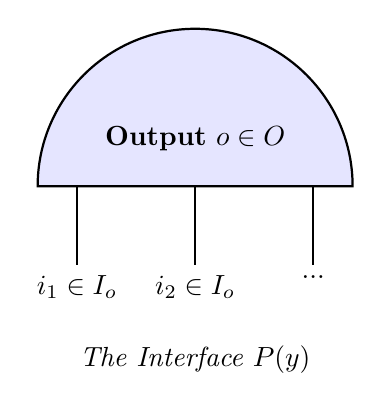
\begin{tikzpicture}
        % The Mushroom Cap (Output/Position)
        \draw[thick, fill=blue!10] (0,1) arc (180:0:2) -- cycle;
        \node at (2, 1.6) {\textbf{Output} $o \in O$};

        % The Stalks (Inputs/Directions)
        \draw[thick] (0.5, 1) -- (0.5, 0) node[below] {$i_1 \in I_o$};
        \draw[thick] (2, 1) -- (2, 0) node[below] {$i_2 \in I_o$};
        \draw[thick] (3.5, 1) -- (3.5, 0) node[below] {$...$};

        % Label
        \node at (2, -1.2) {\textit{The Interface $P(y)$}};
    \end{tikzpicture}
    \caption{A visual representation of a Polynomial Functor (often called a ``Mushroom'' or ``Corolla''). The system offers an Output (the cap) and exposes specific Input ports (the stalks) dependent on that output.}
    \label{fig:poly_mushroom}
\end{figure}

\subsection{The Isomorphism: Genes and Agents}
We now apply this abstract definition to our specific domains.

\begin{definition}[The Gene Object]
A gene $G$ is a polynomial functor where $O_G$ is the set of expressed proteins and $I_G$ is the set of regulatory signals (transcription factors):
\begin{equation}
    P_{Gene}(y) = \sum_{prot \in Proteins} y^{\{TF_{bind}\}}
\end{equation}
\end{definition}

\begin{definition}[The Agent Object]
An autonomous agent $A$ is a polynomial functor where $O_A$ is the set of generated messages, and $I_A$ is the set of observations:
\begin{equation}
    P_{Agent}(y) = \sum_{action \in Actions} y^{\{Obs\}}
\end{equation}
\end{definition}

% ... Continue with "The Interface: Promoters as Lenses" ...

\subsection{The Interface: Promoters as Lenses}

In biology, a gene is not universally accessible. It is guarded by a \textbf{Promoter Region}---a specific DNA sequence that only binds to compatible Transcription Factors. In software, an agent is guarded by an \textbf{API Schema} or Context Window definition.

We model this gating mechanism using \textbf{Optics}, specifically \textbf{Lenses}. A Lens consists of two maps between a global state $S$ and a local view $V$:
\begin{enumerate}
    \item \textbf{Get (View):} $get: S \to V$ (Extracting relevant signal from global state).
    \item \textbf{Put (Update):} $put: S \times V' \to S$ (Updating global state based on local change).
\end{enumerate}

The ``Promoter'' acts as a filter that determines which part of the global cellular environment ($S$) is visible ($V$) to the gene.
\begin{itemize}
    \item \textbf{Biological Lens:} The promoter filters the chaotic cellular soup, allowing the gene to ``see'' only specific molecules (e.g., \textit{Lac Repressor}).
    \item \textbf{Agentic Lens:} The Context Window filters the massive vector database, allowing the agent to ``see'' only the relevant retrieved chunks (RAG).
\end{itemize}

If the input signal does not match the Schema (Promoter), the Lens fails to focus, and the interaction is mathematically undefined (the agent does not run; the gene is not expressed).

\subsection{Epigenetics and State: The Coalgebra}

Neither genes nor agents are stateless functions. They possess memory.
\begin{itemize}
    \item \textbf{Biology:} Epigenetic markers (Methylation, Histone modification) alter how a gene responds to signals without changing the DNA code.
    \item \textbf{Software:} Retrieval Augmented Generation (RAG) and Conversation History alter how an agent responds to a prompt without changing the LLM weights.
\end{itemize}

We model this as a \textbf{Coalgebra} for the polynomial functor $P$. A dynamical system is defined as a tuple $(S, \phi)$, where $S$ is the state space and $\phi$ is the structure map:

\begin{equation}
    \phi: S \to P(S)
\end{equation}

By expanding $P(S)$, we derive the two fundamental operations of the state machine:
\begin{enumerate}
    \item \textbf{Readout:} $S \to O$ (Given current state/memory, what action do I take?)
    \item \textbf{Update:} $S \times I \to S$ (Given current state and new input, what is my new state?)
\end{enumerate}

By establishing this formal dictionary (Table \ref{tab:dictionary}), we assert that GRNs and Agentic Systems are distinct implementations of the same abstract dynamical system.

% --- FIGURE: THE ISOMORPHISM ---
\begin{figure}[h]
    \centering
    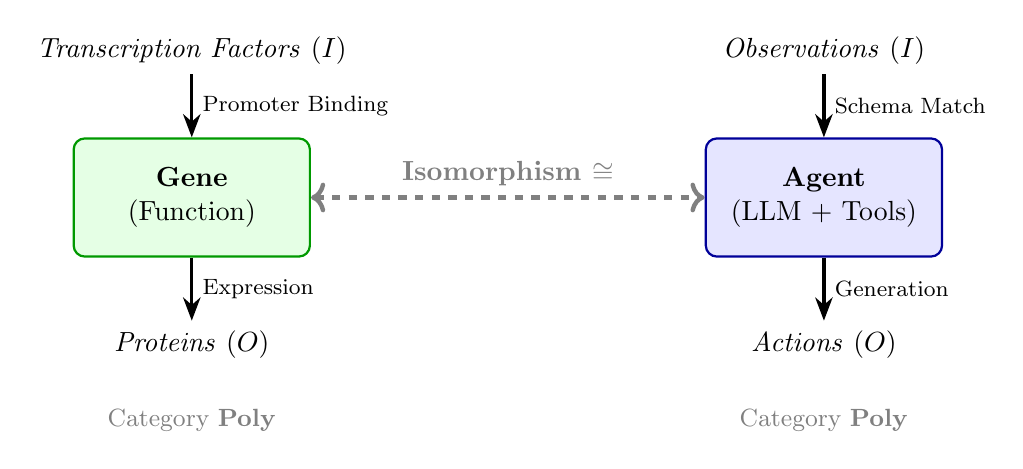
\begin{tikzpicture}[
        node distance=2.5cm,
        box/.style={draw, rectangle, rounded corners, minimum width=3cm, minimum height=1.5cm, align=center, thick},
        arrow/.style={->, >=Stealth, very thick}
    ]
        % Left Side: Biology
        \node[box, fill=green!10, draw=green!60!black] (gene) {\textbf{Gene} \\ (Function)};
        \node[above=0.8cm of gene] (tf) {\textit{Transcription Factors} ($I$)};
        \node[below=0.8cm of gene] (prot) {\textit{Proteins} ($O$)};
        
        \draw[arrow] (tf) -- node[right, font=\footnotesize] {Promoter Binding} (gene);
        \draw[arrow] (gene) -- node[right, font=\footnotesize] {Expression} (prot);
        
        % Right Side: Software
        \node[box, fill=blue!10, draw=blue!60!black, right=5cm of gene] (agent) {\textbf{Agent} \\ (LLM + Tools)};
        \node[above=0.8cm of agent] (obs) {\textit{Observations} ($I$)};
        \node[below=0.8cm of agent] (act) {\textit{Actions} ($O$)};
        
        \draw[arrow] (obs) -- node[right, font=\footnotesize] {Schema Match} (agent);
        \draw[arrow] (agent) -- node[right, font=\footnotesize] {Generation} (act);
        
        % Mapping arrows
        \draw[<->, dashed, ultra thick, color=gray] (gene) -- node[above, font=\bfseries] {Isomorphism $\cong$} (agent);
        \node[below=1.8cm of gene, font=\small, color=gray] {Category $\Poly$};
        \node[below=1.8cm of agent, font=\small, color=gray] {Category $\Poly$};
    \end{tikzpicture}
    \caption{The Structural Isomorphism. Both Genes and Agents act as transducers converting Input Contexts ($I$) into Output Expressions ($O$), governed by the same categorical laws.}
    \label{fig:iso}
\end{figure}

\begin{table}[h]
    \centering
    \renewcommand{\arraystretch}{1.5}
    \begin{tabular}{|l|l|l|}
    \hline
    \textbf{Category Concept} & \textbf{Biological Realization (GRN)} & \textbf{Software Realization (Agentic)} \\ \hline
    Polynomial Functor ($P$) & Gene Interface & Agent Interface (System Prompt) \\ \hline
    Output Position ($O$) & Protein Expression & Tool Call / Message \\ \hline
    Input Direction ($I$) & Transcription Factor Binding & Observation / User Prompt \\ \hline
    Lens (Optic) & Promoter Region & API Schema / Context Window \\ \hline
    Internal State ($S$) & Epigenetic Markers (Methylation) & Vector Store / Chat History \\ \hline
    Morphism ($\circ$) & Signal Transduction Pathway & Data Pipeline \\ \hline
    \end{tabular}
    \caption{The Isomorphism Dictionary}
    \label{tab:dictionary}
\end{table}

% ==========================================
% 4. NETWORK MOTIFS & OPERAD
% ==========================================
\section{Formal Syntax: The Agentic Operad}

To formalize the composition of agents, we define the \textbf{Operad of Wiring Diagrams}, denoted as $\Operad$. An operad can be understood as a ``grammar'' for connecting operations (boxes) via typed wires. It defines which agent topologies are valid and allows us to reason about the properties of the composite system based solely on the properties of its components \cite{vagner2015algebras}.

\subsection{The Typing Rules}
In $\Operad$, every wire carries a specific \textbf{Type} $\tau \in T$.
\begin{equation}
    T = \{ \text{Text}, \text{JSON}, \text{Image}, \text{Error}, \text{ToolCall} \}
\end{equation}

These types correspond to biological molecular specificity (e.g., a specific transcription factor only binds to a specific DNA sequence). A connection is valid if and only if the type of the output port of Agent A matches the type of the input port of Agent B.

\subsection{The Composition Operations}
The operad defines three fundamental operations for combining agents. Any complex agentic architecture, no matter how large, can be decomposed into these three primitives.

\subsubsection{Parallel Composition ($\otimes$)}
Two agents, $A$ and $B$, execute simultaneously with no information exchange:
\begin{equation}
    A \otimes B
\end{equation}
\begin{itemize}
    \item \textbf{Biological Analogy:} Two genes located on different chromosomes expressing proteins independently.
    \item \textbf{Constraint:} This operation is valid only if the internal state spaces $S_A$ and $S_B$ are disjoint. If they share a mutable memory store, the operation leaves the category of polynomial functors and requires a Resource Sharing decorator.
\end{itemize}

\subsubsection{Serial Composition ($\circ$)}
The output of Agent $A$ is piped directly into the input of Agent $B$:
\begin{equation}
    B \circ A
\end{equation}
\begin{itemize}
    \item \textbf{Biological Analogy:} A Signal Transduction Pathway (Protein A activates Protein B).
    \item \textbf{Formal Verification:} This allows for static type checking of agent graphs. If Agent A outputs \texttt{Natural Language} but Agent B expects \texttt{JSON Schema}, the composition is undefined in $\Operad$. This moves runtime hallucination errors to ``compile-time'' architectural errors.
\end{itemize}

\subsubsection{Contraction / Trace ($Tr$)}
A feedback loop where an output port of Agent $A$ is wired back into one of its own input ports:
\begin{equation}
    Tr(A)
\end{equation}
\begin{itemize}
    \item \textbf{Biological Analogy:} Autoregulation (Homeostasis) or Positive Feedback.
    \item \textbf{Software Implication:} This is the topological definition of \textbf{Agency}. A ``stateless'' LLM is a simple morphism. An ``Agent'' is a morphism wrapped in a Trace operation, allowing it to observe its own previous outputs (Chain-of-Thought).
\end{itemize}

\subsection{Theorem: Topological Error Suppression}

We now use this formalism to prove why the \textit{Coherent Feed-Forward Loop} (CFFL) is superior to a direct connection for high-stakes tasks.

\begin{motif}[Coherent Feed-Forward Loop]
A topological structure where Signal $X$ activates $Z$ directly, but also activates $Y$ which gates $Z$. The node $Z$ functions as an AND gate: it fires if and only if $X \land Y$.
\end{motif}

\begin{theorem}[Error Suppression in CFFL]
Let $A_{gen}$ be a generator agent and $A_{ver}$ be a verifier agent. Let $P(E)$ be the probability of a hallucination (error) in any single generation step.

\begin{itemize}
    \item \textbf{Case 1: Direct Link (Serial).} The system fails if $A_{gen}$ hallucinates.
    \[ P(Fail_{direct}) = P(E) \]
    
    \item \textbf{Case 2: CFFL Topology.} The system requires the logical conjunction of the Generator's request ($X$) and the Verifier's approval ($Y$). Assuming the Verifier's error mode is independent of the Generator's (e.g., different prompt strategy or model temperature), the probability that \textit{both} agents simultaneously hallucinate a ``Go'' signal for a destructive action is:
    \[ P(Fail_{CFFL}) = P(E_{gen}) \times P(E_{ver}) \]
\end{itemize}

Since $P(E) < 1$, it follows that $P(E)^2 \ll P(E)$.
\end{theorem}

\begin{proof}
In $\Operad$, the CFFL is defined as a morphism involving a ``Copy'' operation $\Delta_X: X \to X \otimes X$ and an ``AND-Merge'' operation $\mu: Z \otimes Y \to Out$. The existence of the $\mu$ box in the wiring diagram structurally enforces the independence requirement. This proves that safety is a property of the \textbf{topology}, not just the prompt engineering.
\end{proof}

\begin{figure}[h]
    \centering
    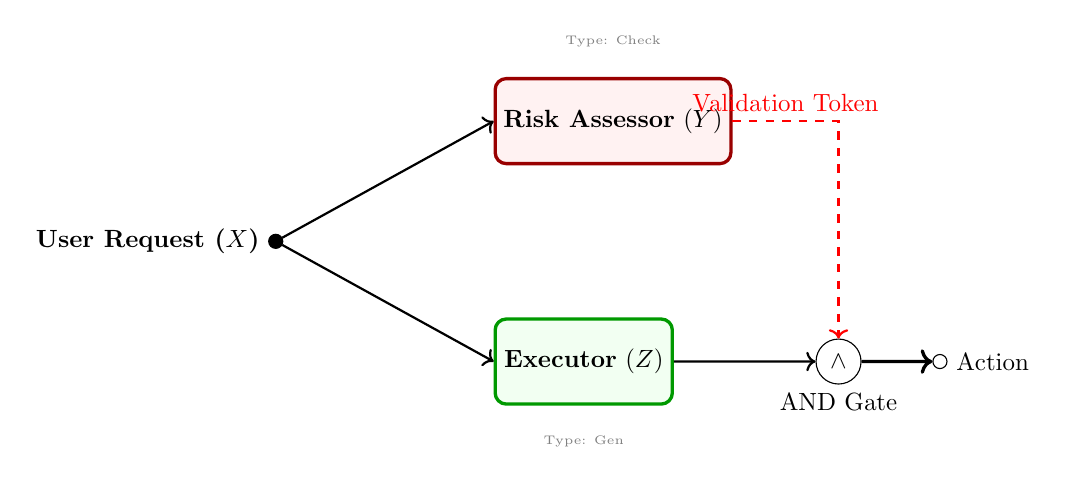
\begin{tikzpicture}[
        node distance=2cm,
        agent/.style={draw, rectangle, very thick, minimum width=2.5cm, minimum height=1.2cm, fill=white, rounded corners},
        input/.style={circle, draw, fill=black, inner sep=2pt},
        output/.style={circle, draw, fill=white, inner sep=2pt},
        scale=0.9, transform shape
    ]
        % Nodes
        \node (in) [input, label=left:\textbf{User Request ($X$)}] {};
        
        \node (assessor) [agent, above right=1cm and 3cm of in, fill=red!5, draw=red!60!black] {\textbf{Risk Assessor} ($Y$)};
        \node (executor) [agent, below right=1cm and 3cm of in, fill=green!5, draw=green!60!black] {\textbf{Executor} ($Z$)};
        
        \node (gate) [draw, circle, right=2cm of executor, label=below:{AND Gate}] {$\land$};
        \node (out) [output, right=1cm of gate, label=right:Action] {};

        % Wires
        \draw[->, thick] (in) -- (assessor.west);
        \draw[->, thick] (in) -- (executor.west);
        
        \draw[->, thick] (executor.east) -- (gate);
        \draw[->, thick, dashed, red] (assessor.east) -| node[near start, above] {Validation Token} (gate.north);
        
        \draw[->, very thick] (gate) -- (out);
        
        % Annotations
        \node[above=0.3cm of assessor, font=\tiny, color=gray] {Type: Check};
        \node[below=0.3cm of executor, font=\tiny, color=gray] {Type: Gen};

    \end{tikzpicture}
    \caption{The CFFL implemented in $\Operad$. The Executor ($Z$) cannot act without the token from the Risk Assessor ($Y$), topologically preventing unilateral hallucinations.}
    \label{fig:cffl}
\end{figure}

\subsection{Quorum Sensing (Consensus \& Voting)}

\begin{motif}[Quorum Sensing]
A distributed topology where multiple agents emit a weak signal $\sigma$ into a shared environment. An effector node $E$ activates if and only if the concentration $[\sigma] > \theta$.
\end{motif}

\begin{itemize}
    \item \textbf{Biological Function:} Many bacteria (e.g., \textit{V. fischeri}) secrete auto-inducer molecules. Individual bacteria do not react to low concentrations. However, once the population density reaches a threshold (Quorum), the concentration of auto-inducers triggers a simultaneous, coordinated gene expression event (e.g., bioluminescence or biofilm formation).
    \item \textbf{Agentic Isomorphism (Voting Ensembles):} In non-deterministic systems, a single agent's output is noisy. By instantiating $N$ parallel agents (a \textbf{Mixture of Experts}), the system aggregates their outputs. The final action is taken only if the ``concentration'' of a specific semantic token exceeds a confidence threshold. This transforms weak, noisy individual signals into a robust, high-confidence collective action.
\end{itemize}

\subsection{Chaperone Proteins: Output Structural Validation}
\begin{itemize}
    \item \textbf{Biological Function:} Newly synthesized proteins emerge as linear chains that must fold into precise 3D structures to function. \textbf{Chaperone Proteins} (e.g., GroEL-GroES) sequester unfolded proteins, preventing aggregation and facilitating correct folding. If a protein fails to fold repeatedly, it is tagged for degradation (Ubiquitination) to prevent toxic buildup.
    \item \textbf{Agentic Isomorphism (Retry \& Repair Loops):} Generative models output unstructured token streams (``linear chains''). However, downstream agents require strictly structured inputs (e.g., valid JSON Schemas). A \textbf{Validator Agent} acts as a Chaperone: it intercepts the raw output, attempts to parse it into a formal schema (``folding''), and if validation fails, returns the error trace to the generator for re-synthesis. This turns a probabilistic string into a deterministic data structure.
    \item \textbf{Categorical View:} The Chaperone acts as a \textbf{Retraction} map $r: S \to V$ from the free monoid of text to the structured type $V$, such that $r \circ i = id_V$.
\end{itemize}

% ==========================================
% 5. FAILURE MODES (PATHOLOGY)
% ==========================================
\section{Failure Modes \& Pathology}

A key insight of Systems Biology is that diseases are often not caused by the complete failure of a single component, but by the \textbf{dysregulation of network dynamics}. A cancerous cell still ``works''---in fact, it works too well, reproducing indefinitely. Similarly, catastrophic failures in agentic systems often arise from functional agents interacting in topologically pathological ways.

We classify three primary classes of agentic pathology based on their biological isomorphisms.

\subsection{Oncology: Infinite Loops as Unchecked Growth}
\begin{itemize}
    \item \textbf{Biological Pathology (Cancer):} In a healthy cell, the cell cycle is driven by a positive feedback loop (Cyclins) but constrained by negative feedback ``checkpoints'' (e.g., the p53 gene). If p53 is mutated, the negative feedback is severed. The positive loop runs unchecked, leading to exponential proliferation (tumor growth).
    \item \textbf{Agentic Pathology (The Recursive Hang):} Two agents get stuck in a politeness loop (e.g., ``Thank you,'' ``You're welcome'') or a debugger agent continuously generates new bugs to fix old ones.
    \item \textbf{Categorical Diagnosis:} The Trace operation $Tr(A)$ lacks a \textbf{Contractive Map} property. In the metric space of the conversation, the distance between state $S_t$ and $S_{t+1}$ approaches zero ($d \to 0$), but the system fails to trigger a ``Stop'' token.
    \item \textbf{Treatment:} Implementation of an \textit{Apoptosis} (Cell Death) mechanism. A meta-monitor agent observes the \textit{entropy} of the conversation. If information gain drops below a threshold (the conversation becomes repetitive), the monitor forces a termination signal.
\end{itemize}

\subsection{Autoimmunity: Hallucination Cascades}
\begin{itemize}
    \item \textbf{Biological Pathology (Autoimmune Disease):} The immune system relies on distinguishing ``Self'' (internal tissue) from ``Non-Self'' (foreign pathogens). In diseases like Lupus, this distinction blurs, and the system attacks healthy tissue.
    \item \textbf{Agentic Pathology (Context Poisoning):} Agent A hallucinates a fact (e.g., a non-existent library function). Agent B reads this hallucination from the shared history, treats it as ground truth, and builds complex logic upon it. The error amplifies through the network until the output is detached from reality.
    \item \textbf{Categorical Diagnosis:} A failure of the \textbf{Lens} to distinguish source types. The input port $I$ accepts both \texttt{External\_Observation} (User/Tool) and \texttt{Internal\_Memory} (History) without distinction.
    \item \textbf{Treatment:} Strict Schema Typing. We must distinguish ``Self'' (Generated Tokens) from ``Non-Self'' (Tool Outputs) at the schema level. The Reviewer Agent should weigh \texttt{Tool\_Output} with higher authority than \texttt{Agent\_Thought}.
\end{itemize}

\subsection{Prion Disease: Topological Corruption via Prompt Injection}
\begin{itemize}
    \item \textbf{Biological Pathology (Prions):} Unlike viruses, prions lack genetic material. They are misfolded proteins that induce conformational changes in healthy proteins upon contact, triggering a chain reaction of structural corruption (e.g., Creutzfeldt-Jakob disease).
    \item \textbf{Agentic Pathology (The Jailbreak Cascade):} A malicious string (Prompt Injection) enters the Context Window. The agent, attending to this string, ``misfolds'' its alignment, outputting a compliant response to a harmful query. If this output is fed into a downstream agent, the ``infection'' propagates purely through the geometry of the embedding space, without valid authorization.
    \item \textbf{Categorical Diagnosis:} A violation of \textbf{Information Flow Security} within the Operad. The injection acts as a \textit{topological defect} that bypasses the Schema/Lens filter by mimicking the structure of a trusted signal.
    \item \textbf{Treatment:} \textbf{Denaturation Layers}. Implementing an intermediate transformation layer (e.g., paraphrasing or sanitization) between agents that disrupts the specific syntax (folding) required for the injection to work, rendering the ``prion'' inert.
\end{itemize}

\subsection{Ischemia: Resource Exhaustion}
\begin{itemize}
    \item \textbf{Biological Pathology (Ischemia):} A tissue may be genetically perfect, but if blood flow (oxygen/ATP) is restricted, metabolic processes stall, leading to necrosis.
    \item \textbf{Agentic Pathology (Token Starvation):} An agentic graph is logically sound but fails mid-execution because the context window is full or the API rate limit is hit.
    \item \textbf{Categorical Diagnosis:} A failure in the \textbf{Resource Functor}. Every operation in the Operad carries a cost ($c$).
    \begin{equation}
        \sum_{agent \in Graph} Cost(agent) > Budget
    \end{equation}
    \item \textbf{Treatment:} \textbf{Metabolic Regulation}. Instead of a fixed loop, implement ``Budget-Aware'' agents. The agent observes its own remaining token count (ATP levels) and dynamically simplifies its reasoning strategy (switching from Chain-of-Thought to Zero-Shot) to conserve energy.
\end{itemize}

% ==========================================
% 6. DISCUSSION
% ==========================================
\section{Discussion: Towards ``Epigenetic'' Software}

The isomorphism presented in this paper extends beyond the immediate execution of tasks (Gene Expression) to the management of long-term behavior and state. In biology, the DNA sequence is static; a neuron and a liver cell possess the exact same genetic code. Their distinct behaviors are determined by \textbf{Epigenetics}---chemical markers (like methylation) that restrict access to certain parts of the genome, effectively biasing the system toward specific outcomes.

\subsection{RAG as Digital Methylation}
In Agentic Systems, the Large Language Model (LLM) weights act as the DNA---a static, pre-trained substrate of potentiality. To create specialized agents, we do not typically retrain the model (mutation); instead, we use \textbf{Retrieval Augmented Generation (RAG)} and System Prompts.

We define this formally as \textbf{Phenotypic Plasticity}. The output of an agent is not solely a function of its weights ($W$) and the user query ($Q$), but of its epigenetic state ($E$):
\begin{equation}
    O_{agent} = f(W, E, Q)
\end{equation}

Context injection (RAG) acts as a \textbf{restrictive morphism}. By populating the context window with specific documents (e.g., ``SQL Syntax Guide''), we effectively ``methylate'' (silence) the vast majority of the LLM's general knowledge (e.g., poetry, history) to force the expression of a specific ``SQL Agent'' phenotype.

This suggests that the \textbf{State Monad} for an agentic system should not merely be a log of messages, but a structured \textit{Epigenetic Landscape} that strictly controls which ``genes'' (capabilities) are accessible at any given step in the workflow.

\subsection{Horizontal Gene Transfer: Dynamic Tool Loading}
Standard evolution relies on vertical inheritance (Pre-training). However, bacteria utilize \textbf{Horizontal Gene Transfer} (HGT) to acquire new capabilities (Plasmids) from the environment in real-time. 

In Agentic Systems, we map Plasmids to \textbf{Tool Schemas}. An agent operating in a novel environment may encounter a problem for which its ``genomic'' (pre-trained) capabilities are insufficient. 
\begin{equation}
    Agent_{new} = Agent_{old} \otimes Tool_{Schema}
\end{equation}
By dynamically retrieving a tool definition (e.g., a Calculator API or SQL Interface) from a registry and injecting it into the Context Window, the agent undergoes a topological transformation, acquiring a new input/output modality instantly. This suggests that robust agentic architectures should support a ``Plasmid Registry''---a marketplace of ephemeral tools that agents can ingest and discard as needed.

\subsection{The Cost of State: The Metabolic Bound}
Every biological process is constrained by ATP availability. Similarly, every agentic operation is constrained by token limits and latency. We propose that future agentic frameworks must implement the \textbf{Resource Functor} $R$ at the kernel level:
\begin{equation}
    R(Agent): (Inputs, Budget) \to (Outputs, RemainingBudget)
\end{equation}

An agent graph should be ``compiled'' with a guaranteed upper bound on token consumption. If the topological structure allows for an unbounded loop (Unchecked Growth), the compiler must reject the architecture before deployment, much like a cell undergoes apoptosis if metabolic stress becomes critical.

\subsection{Endosymbiosis: The Neuro-Symbolic Integration}
The evolution of complex life was triggered by \textbf{Endosymbiosis}, where a host cell engulfed a bacterium (the future Mitochondrion), gaining the ability to generate massive energy (ATP) via aerobic respiration. This represents the integration of two distinct metabolic substrates.

In Agentic AI, this maps to the integration of \textbf{Connectionist} (Neural) and \textbf{Symbolic} (Code) subsystems. An LLM acts as the host organism---capable of planning and semantic reasoning but energetically inefficient at arithmetic and logic. By ``engulfing'' a deterministic runtime (e.g., a Python REPL or Wolfram Engine), the agent delegates high-precision tasks to the symbolic organelle.
\begin{equation}
    Agent_{Eukaryote} = LLM_{Host} \oplus Runtime_{Mitochondria}
\end{equation}
Just as the host cell provides nutrients to the mitochondria in exchange for ATP, the LLM provides parsed variables to the runtime in exchange for deterministic truth.

% ==========================================
% 7. CONCLUSION
% ==========================================
\section{Conclusion}

The transition from ``Prompt Engineering'' to ``Agentic Engineering'' represents a shift from alchemy to chemistry. However, current methodologies remain fragile, relying on trial-and-error prompting rather than rigorous architectural principles.

In this paper, we have demonstrated that \textbf{Gene Regulatory Networks (GRNs)} provide a proven architectural blueprint for distributed, stochastic information processing. By formalizing this analogy through \textbf{Applied Category Theory}, we have derived a suite of robust design patterns:

\begin{enumerate}
    \item \textbf{Robustness:} The use of \textit{Quorum Sensing} and \textit{CFFL} topologies to filter stochastic noise.
    \item \textbf{Validity:} The use of \textit{Chaperone Proteins} to enforce structural determinism on probabilistic outputs.
    \item \textbf{Security:} The identification of \textit{Prion-like} prompt injections and the topological defenses required to stop them.
    \item \textbf{Evolution:} The mapping of \textit{Horizontal Gene Transfer} to dynamic tool loading and \textit{Endosymbiosis} to neuro-symbolic integration.
\end{enumerate}

We conclude that the future of reliable AI agents lies in \textbf{biomimetic topology}. By structuring our software according to the logic of life---from the metabolic constraints of Ischemia to the symbiotic integration of code and intuition---we inherit the billions of years of R\&D that biology has invested in solving the problem of autonomous control.

\newpage

% ==========================================
% REFERENCES
% ==========================================
\printbibliography

\end{document}
